
The above equations can be expressed as the matrix equation
\begin{align}
     \myvec{3&2\\2&-3}\vec{x}=\myvec{5\\7}
\end{align}
The augmented matrix for the above equation
is row reduced as follows
\begin{align}
     \myvec{3& 2& 5\\
           2 & -3 & 7}
          \xleftrightarrow{R_1 \leftarrow\frac{1}{3}{R_1}}
    \myvec{1&\frac{2}{3}&\frac{5}{3}\\
        2&-3&7}\\
        \xleftrightarrow{R_2\leftarrow  -2R_1+R_2}
    \myvec{1&\frac{2}{3}&\frac{5}{3}\\0&\frac{-13}{3}&\frac{11}{3}}\\
    \xleftrightarrow{R_2\leftarrow \frac{-3}{13}{R_2}}
    \myvec{1&\frac{2}{3}&\frac{5}{3}\\0&1&\frac{-11}{13}}\\
    \xleftrightarrow{R_1\leftarrow \frac{-2}{3}R_2+R_1}
    \myvec{1&0&\frac{29}{13}\\0&1&\frac{-11}{13}}
    \end{align}
resulting in 
 \begin{align}
     \myvec{3&2&5\\2&-3&7}
 \end{align}
with 2 nonzero rows. So it's rank is 2. The rank of the following matrix is also 2.
   \begin{align}
       \myvec{3&2\\2&-3}
   \end{align} 
 %  
   $\therefore$ lines are consistent and give a unique solution.
%
\begin{figure}[!ht]
\centering
    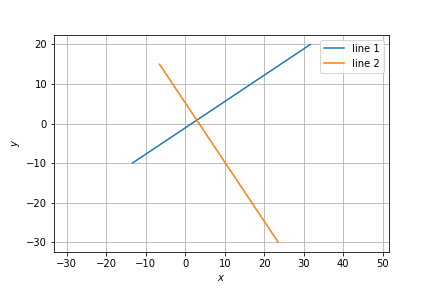
\includegraphics[width= \columnwidth]{solutions/sep/2/5/a/consistent.png}
    \caption{Graphical solution}
    \label{sep/2/5/a/Fig:Graphical Solution}
\end{figure}

This is verified in Fig.     \ref{sep/2/5/a/Fig:Graphical Solution}.
